\documentclass[a4paper,10pt]{article}

\usepackage[latin1]{inputenc}
\usepackage{epsfig}
\usepackage{graphicx}
\usepackage{url}
\usepackage{times}
\usepackage{rotating}

\begin{document}

\title{Exercise 1: Software Architecture Description of the HS07 System}

\author{
  Anders H Poder, Jesper Dalberg, Lars Kringelbach\\\\
  Department of Computer Science, University of Aarhus\\
  Aabogade 34, 8200 {\AA}rhus N, Denmark\\\\
  \makeatletter
  \texttt{Group 11 - Kilo}\\
  \texttt{19951439, 20074976, 20074842}\\
  \texttt{\{ahp, jdalberg, u074842\}@daimi.au.dk}
}

\date{2008-02-04 13:32}

\maketitle

% =====================================================================
\begin{abstract}
  The HS07 system implements a closed-loop control of the heating in a
  private home. It monitors thermometers in the home, and based on
  measurements HS07 adjusts radiators in the home. This report gives a
  software architecture description of an architectural prototype of
  the HS07 system. The techniques used for architectural description
  are taken from \cite{christensen2004archdesc}.
\end{abstract}

% =====================================================================
\section{Introduction}

Figure~\ref{fig:hs07} shows a schematic overview of HS07 in a
home. The home may be accessed by the home owner from the outside
through the HS07 gateway. The HS07 gateway also monitors and controls
the home.
\begin{figure}[!htb]
\centerline{\epsfig{figure=figures/hs07,scale=0.4 }}
\caption{HS07 in a home}
\label{fig:hs07}
\end{figure}

HS07 includes sensor and actuator hardware which runs on an embedded Java virtual
machine with standard software.

% =====================================================================
\section{Architectural Requirements}

For our purposes there is one main use case for the HS07 system:
\begin{quote}
  \emph{Control Temperature}: The gateway collects measurements from
  thermometers and reports this to radiators that then control the
  temperature.
\end{quote}

The major driving qualities attributes of the HS07 system
are\footnote{These qualities will be operationalized in Exercise 2}:

\begin{itemize}
\item \emph{Performance.} HS07 should be performant so that a large
  number of thermometers and radiators may be part of the system.
\item \emph{Modifiability.} It must be possible to modify HS07 to
  include new types of sensors and actuators.
  \item $<<$Extra quality requirement that you consider important $>>$
\end{itemize}


% =====================================================================
\section{Architectural Description}

% ---------------------------------------------------------------------
\subsection{Module Viewpoint}

The module viewpoint of the HS07 system.

\begin{figure}[!htb]
\center {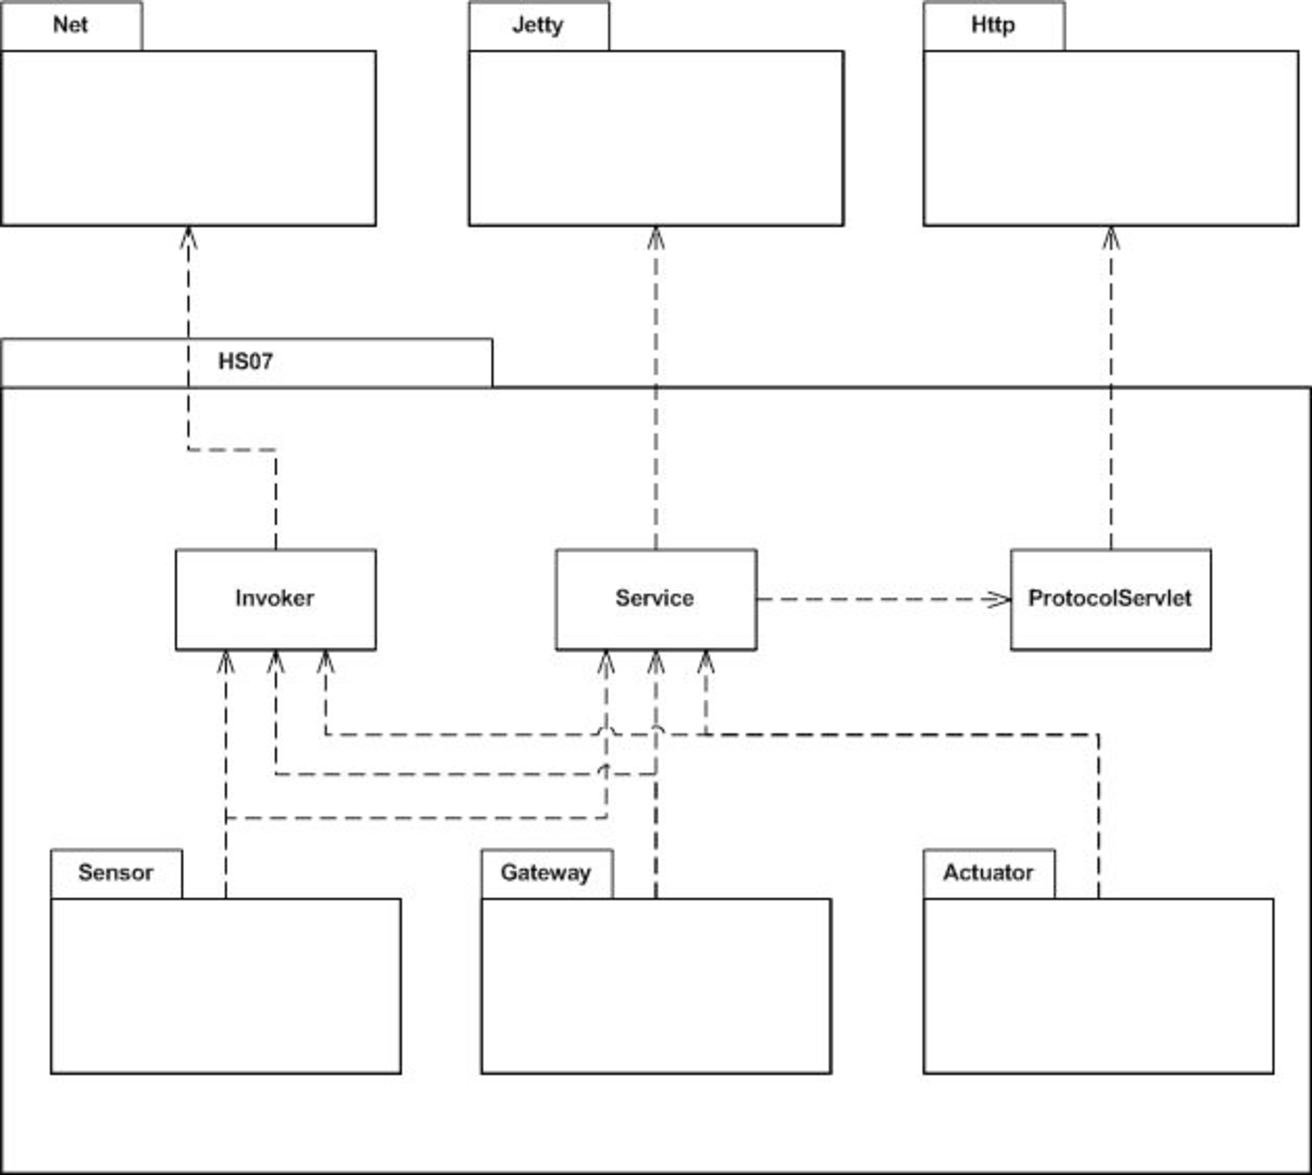
\includegraphics[viewport=0 10 600 500,scale=0.5]{figures/mv.pdf}}
\caption{HS07 Package Diagram}
\label{fig:mv}
\end{figure}

The figure shows the packages of the HS07 system, and how they interact 
with java packages used.

% ---------------------------------------------------------------------
\subsection{Component \& Connector Viewpoint}

The Component \& Connecter view consists of an Active Objects diagram and a
sequence diagram. The Active Objects diagram shows the active objects of 
the HS07 system, and how they interact. 

\begin{figure}[!htb]
\center {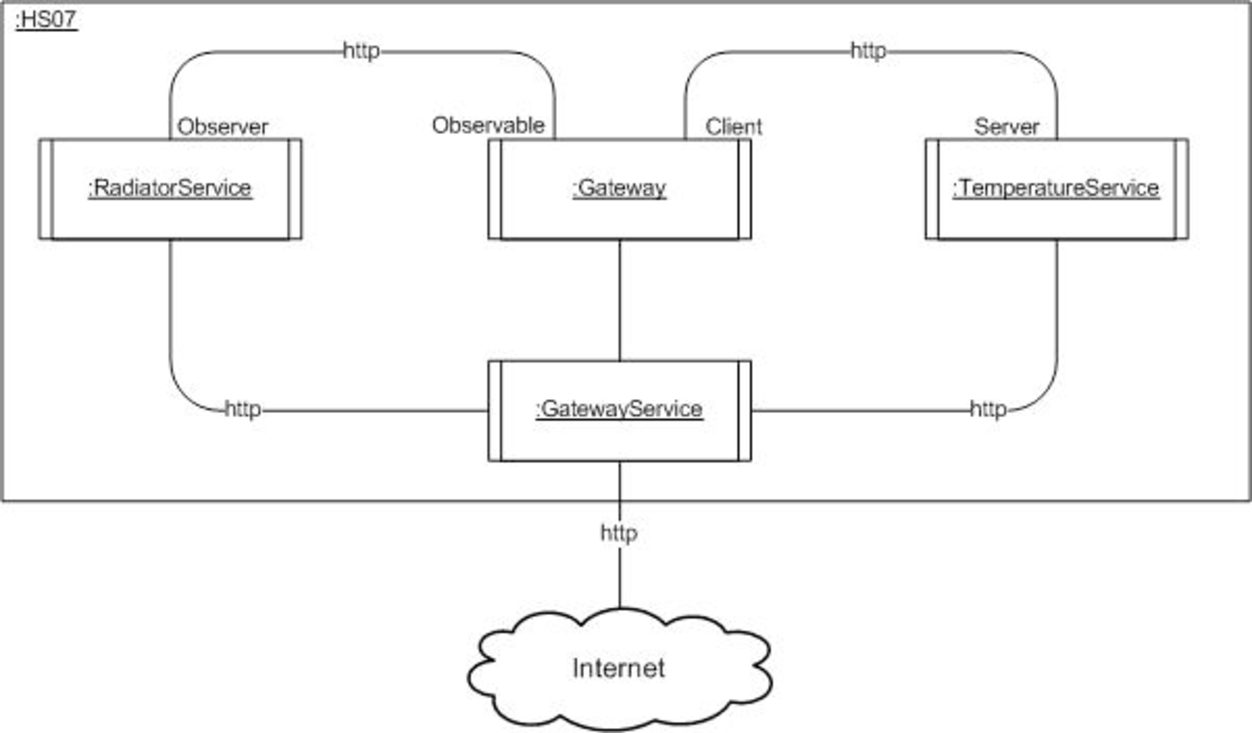
\includegraphics[viewport=0 10 600 420,scale=0.5]{figures/cc_ao.pdf}}
\caption{HS07 Active Objects}
\label{fig:cc_ao}
\end{figure}
The sequence diagram illustrates the protocol of the interactions involved in the setup and the execution of the Gateway. It consists of a registration sequence and an infinite loop of retrieving the temperature of all registered themometers and nitifying all observers (in this case the Radiators). The example is slightly simplified to improve readability, as the registerThermometer, registerObserver, getTemperature and notify is actually network calls performed using the Invoker and the respective servers.
\begin{figure}[!htb]
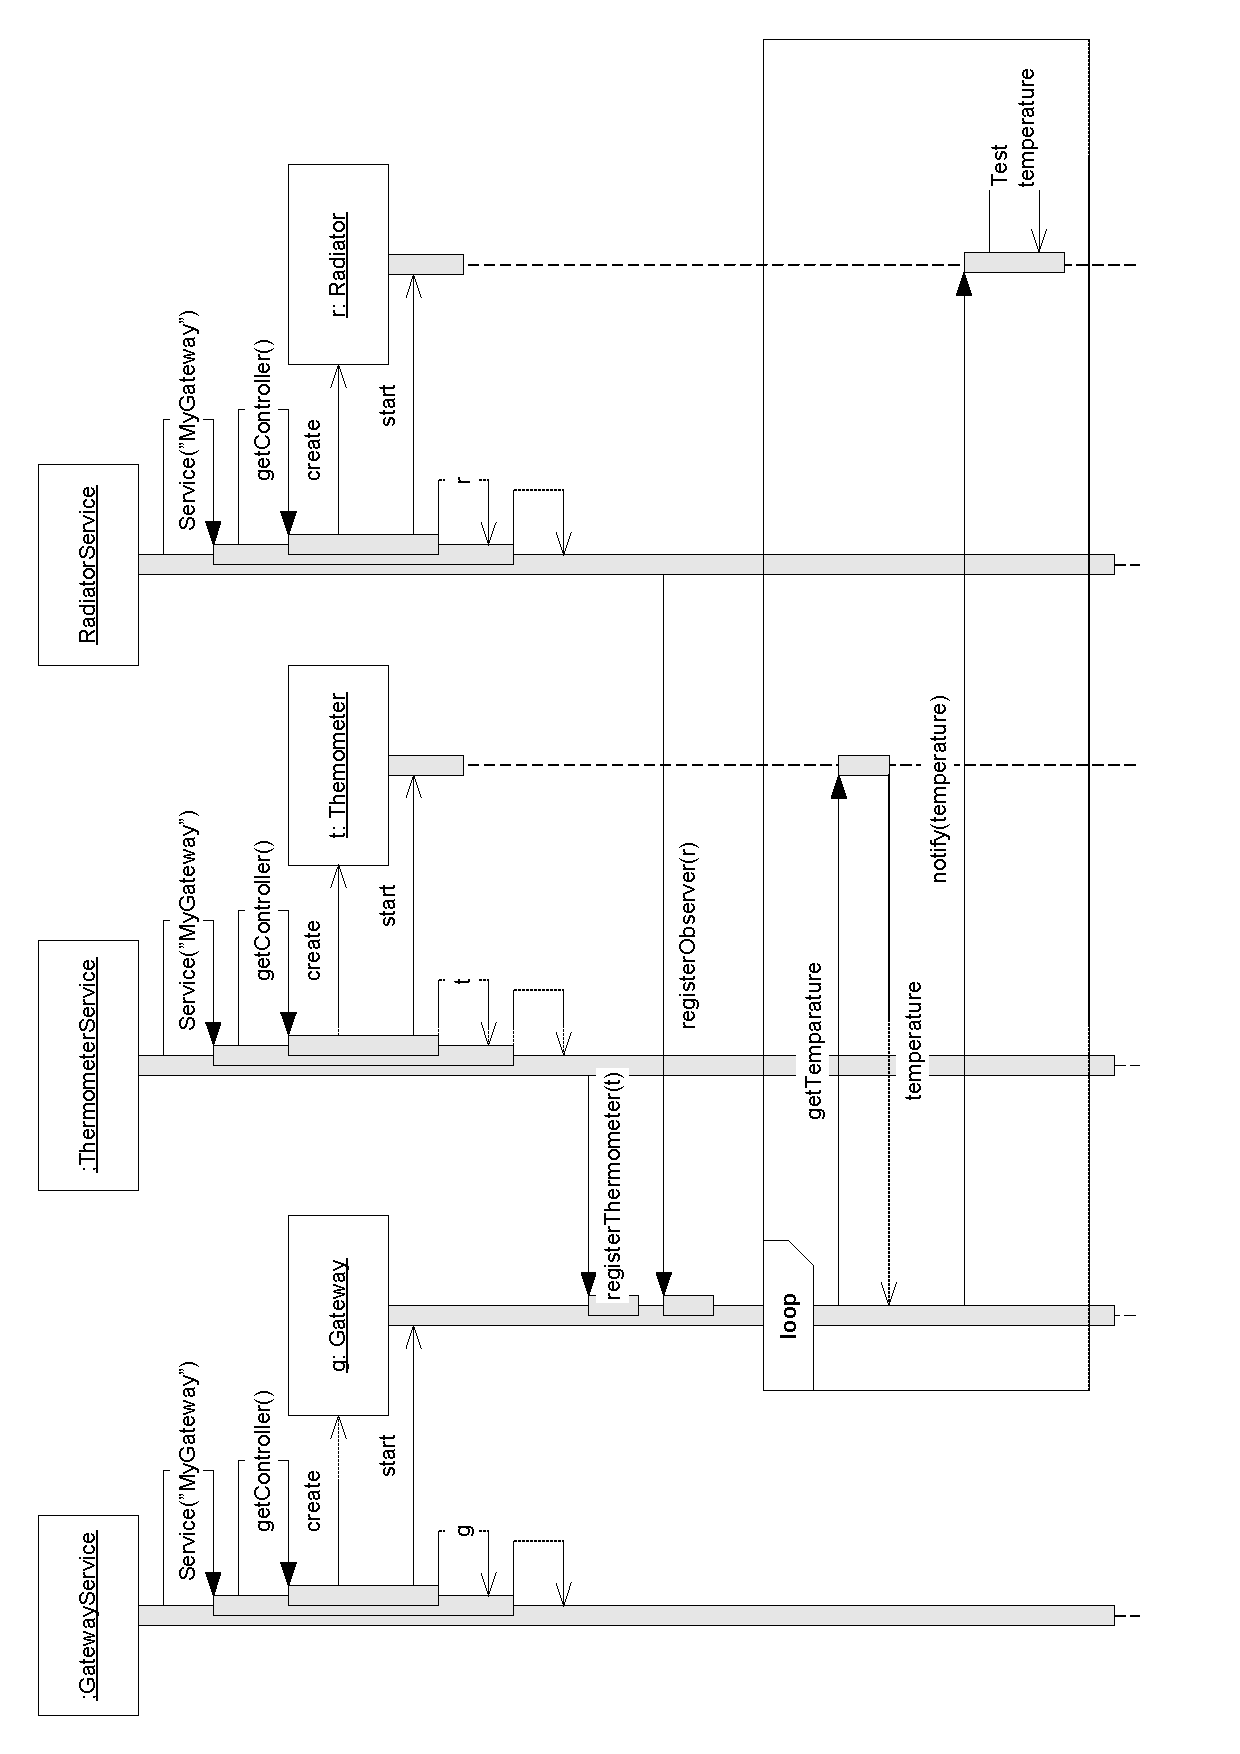
\includegraphics[angle=90,scale=1.2]{figures/sequence.pdf}
\caption{HS07 Sequence Diagram}
\label{fig:sequence}
\end{figure}
\clearpage


% ---------------------------------------------------------------------
\subsection{Allocation Viewpoint}

The allocation viewpoint illustrates how components are deployed in actual processes
within the HS07 system.

\begin{figure}[!htb]
\center {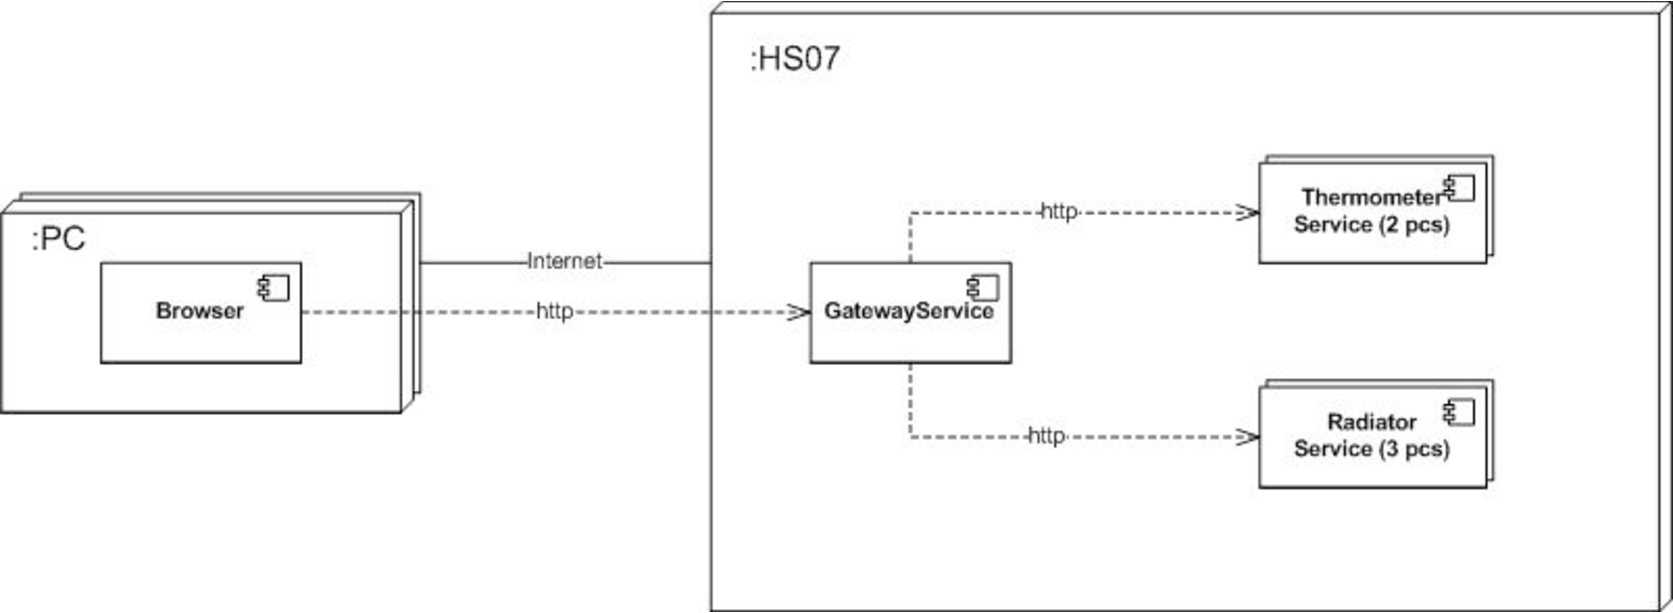
\includegraphics[viewport=0 10 700 350,scale=0.4]{figures/deployment.pdf}}
\caption{HS07 Allocation Diagram}
\label{fig:allocation}
\end{figure}


% =====================================================================
\section{Discussion}
\subsection{Strength and Limitations of the approach}
$<<$What are the strengths and limitations of this approach to
architectural description judging from this case?$>>$

When using the approach described in \cite{christensen2004archdesc} with reverse 
engineering to achieve an architectural description, the dangers posed seem to 
be finding the correct balance in the choice of detail level. It
is easy to get to much information, cluttering the purpose of the 
AD, which in a basic sense is to clarify and present at wider understanding of
the system.

Experienced architects might recognize patterns emerging from the process, and 
immediately see possible design flaws in the implementation of these, thus
being able to help improve the quality of any evolving system.

The purpose of doing a reverse engineered AD must either be to evolve
the system of to extract clarification. Care should be taken to achieve either
goal. 
\subsection{Whats missing?}
$<<$Are there aspects of the software architecture that have not been
properly described?$>>$
Stakeholders and their concerns. This encompasses both users/aquirers and developers. We also need to discuss the feasibility and maintainablity of the system. 

\subsection{IEEE Conformance}

$<<$For the architectural description above, discuss what (if anything) should be changed or added for it to comply with the IEEE recommended practice for architectural description$>>$

The following are the problems identified in order to comply with \cite{ieeerecommendedpractice}.

Clause 5.2: The stakeholders and their precise concerns need to be identified for each view. 

Clause 5.5: Consistency checks across all existing views.

\subsection{Perry \& Wolf Considerations}
$<<$Consider the definition of software architecture by [Perry and Wolf, 1992]. Discuss what the 'elements', 'form', and 'rationale' according to this definition would be for the HS07 system$>>$

\cite{perrywolf1992} defines "elements" as three different classes, data elements, processing elements and connecting elements. In HS07 the data elements are temperatures, the processing element is the gateway and the connecting element is HTTP. The "form", as described by Perry and Wolf, is the choice of the observer pattern in HS07, and the "rationale" for doing so are defined by the Achitectural Requirements described elsewhere in this document.

% =====================================================================
\section{...}

% =====================================================================
\bibliography{paper}
\bibliographystyle{apalike}


\end{document}
